\documentclass[12pt]{article}
\usepackage[utf8]{inputenc}
% \usepackage[english]{babel}
%\usepackage{helvet}
\usepackage{graphicx}
\usepackage{hyperref}
\usepackage{natbib}
\usepackage[inline, shortlabels]{enumitem}
\RequirePackage[a4paper,top=3.5cm,left=3cm,right=3cm,bottom=2.4cm]{geometry}
\title{Sidepit: Fair Price Discovery via Decentralized Exchange}
\author{Yehuda Jay Berg \\jaybny@gmail.com}
\date{May 2021}

\begin{document}
\parindent 0cm
\parskip   6pt
\maketitle

% \documentclass[a4paper]{article}

% \setlength\parindent{0pt}

% \begin{document}

% \title{Sidepit}
% \maketitle
\begin{abstract}
Ever since Satoshi solved peer to peer digital cash with Bitcoin, people have been trying to apply similar techniques to solve other hard problems. One such problem, peer to peer exchange, is one of the most difficult of these problems. An exchange is a financial market, where trading of securities occurs. The purpose of an exchange is twofold; 1) for price discovery, 2) for counter-party settlement. Centralized Exchanges have been well researched and developed in traditional finance for well over a century. They evolved from trading under a tree, to the Chicago trading pits, to electronic exchanges with continuous limit order books. Modern exchanges provide 24/7 trading, and offer co-location for the most prolific traders, high frequency trading bots. Decentralized exchanges aim to bring traditional centralized exchanges into a peer-to-peer blockchain protocol. Due to early bitcoin exchange hacks, most research has been focused on the settlement utility of exchange. We focus on the price discovery utility, an emergent property of real-time trading. We present Sidepit fair price discovery with decentralized exchange by solving the impossible task of consensus on total ordering of transactions to mitigate front-running. 
\end{abstract}

\section*{Introduction}

\paragraph*{Price discovery}is a social benefit and a key goal in the design of a market structure. In fact, the goal of the architecture of an exchange mechanism, is to attract as much liquidity needed for price discovery.  \cite{francioni_schwartz_2017}

Price discovery is described in microstructure research as a search for an equilibrium price based on new external information. This new information is reflected in the traders orders, and is ultimately converted into a market price. \citep{RePEc:nbr:nberwo:6257}

Some even define an exchange as ``any trading facility that has as its primary function the delivery of good price discovery'' \cite{francioni_schwartz_2017}. 

Price discovery is the dynamic process of market prices moving from the old equilibrium to a new one, based on new information. The price discovery utility of exchange and its importance as a social good, is often overlooked, mostly due to the non-observability of equilibrium prices, making it difficult to quantify. \cite{francioni_schwartz_2017} \cite{RePEc:udb:wpaper:uwec-2005-01-r} 


\paragraph*{Limit order books} and price discovery are tightly related. \citep{RePEc:nbr:nberwo:6257} \cite{RePEc:eee:jfinec:v:17:y:1986:i:1:p:5-26}

To achieve price discovery exchanges offer two order types. Limit orders, and Market orders. All orders are sent to a centralized matching engine in the exchange servers. 

Market orders have a quantity but no price. 

\begin{enumerate*}
    \item "Buy 1 @ market" - an order to buy 1 unit of the asset at the market  
\end{enumerate*}

Limit orders have a quantity and a price. 

\begin{enumerate*}
    \item "Buy 1 @ 100" - an order to buy 1 unit of the asset at the market  
\end{enumerate*}


\paragraph*{Continuous limit order book (CLOB)}is the market micro structure that leads to price discovery \footnote{Other types of markets such as call auctions, and dealer markets, do not provide the robustness of limit orders for price discovery. \cite{RePEc:hal:journl:hal-00459785}}. There are two order types. Limit orders, where you provide your own price, with the risk of waiting to be matched, and market-orders, where you get filled immediately in return for a possibly worse price.

The interaction where market orders match limit orders is continuous. 

The state of a CLOB in a centralized exchange is shown to produce a price discovery equilibrium. 

For the purpose of price discovery, the match of buyers and seller must be atomic, or one party can pull out of the deal after the fact. 

\subsubsection*{Evolution of Exchange}
The design of CLOB evolved from previous exchanges. Futures trading pits in Chicago reached price discovery equilibrium.  

Before electronic markets, an open outcry system in physical trading pits were setup at the exchange place. Buyers and sellers would be bunched up near each other, and they would verbalize their intention to buy or sell, the quantity they wish to trade, and the price they are willing to accept or pay. Traders would seek out the best prices by verbally matching with their counter-parties. 

\textbf{A match in a trading pit is the real atomic swap.} 

For the purpose of Price Discovery what needs to be atomic is the match, otherwise one party can pull out of the deal. Centralized exchanges, like CME, provide this guarantee. 

\textbf{Atomic swap DEXs, that allow one side to back out does not provide price discovery.}

Backing out of a trade is the most used move by participants in modern exchanges. In fact, 60\%  of all orders placed on centralized exchanges are cancelled within 1 millisecond.  

Going electronic, exchanges were faced with asynchronous message over IP. No longer can buyers and sellers interact simultaneously. Market makers in NASDAQ and specialist in NYSE were tasked with providing liquidity and filling orders. 

Exchanges added anti-front-running rules, so for-profit MMs did not abuse the system. Rules, such as Reg NMS were made, not to prevent front-running, but to ensure price discovery.

Early market maker based electronic exchanges, such as NASDAQ, were facing problems analogous to the problem of Miner Extracted Value (MEV) we see in Ethereum today. Where miners can not only front-run but can also add their own orders after seeing everyone else's. Exchanges feared this would lead to loss of confidence in the market which would affect the fragile state where the equilibrium of price discovery exists. 

When designing a DEX, we keep in mind how obvious unfairness will ultimately hurt liquidity, the exchange overall, and Price Discovery in particular. In fact, the main issue with decentralized CLOB is not the MEV or front-running but the loss of confidence stemming from those problems.  


\subsubsection*{The HFT Problem}
\textbf{The reason 60\% of all ordes are immediately canceled in today's markets is due to adverse selection risk of stale limit orders.} 

At the turn of the 21st century, exchanges adopted  Continuous Limit Order Books (CLOBs). No more specialist front-running or market-makers. They were replaced with High Frequency Market Makers (HFT-MM) 

High Frequency refers to the reaction time of automated trading bots. This reaction time determines how often you are incentivized to cancel your orders. 

Unless you are the absolute fastest, you are incentivized to immediately cancel your market making orders due to \emph{Adverse Selection Risk} (ASR)  

Example: \( reaction time = 2 seconds \) 

$t_0$ limit buy 1 \$IBM @ 100 \\
$t_2$ IBM files bankruptcy 

At $t_0$ you place limit order to buy 1 share of IBM at \$100, and at $t_2$ you learn that IBM has filed bankruptcy, and you immediately cancel. However at $t_2$ your adversary also hears the news, and sends a sell order to attempt to fill you. Its a classic race, fill vs cancel.

$t_2$ Hero send cancel order to exchange  \\
$t_2$ Villan send sell 1 \$IBM @ market  

Since the Villan's reaction time is only 1 second while yours is 2 seconds, his orders hits the matching engine at $t_3$ , while Hero's cancel doesn't get there until $t_4$. Hero ends up buying IBM after learning they filed bankruptcy! This is an example of \emph{Adverse Selection Risk} (ASR). In fact, all limit orders sitting on the book are subject to ASR. Special \emph{HFT Bandit} bots, are designed just to snip these "stale" limit orders. 

$t_0$ limit buy 1 \$IBM @ 100 \\
$t_1$ cancel \\
$t_2$ if ( no bad news ) limit buy 1 \$IBM @ 100 \\
$t_3$ cancel 

If instead your trading plan was to \emph{flash} all your orders, by sending and immediately canceling. You would have already canceled at $t_1$ and after learning about the bankruptcy, you wouldn't have sent the new buy order at $t_2$

The objective of the Market Maker is to buy at bid and sell at ask repeatedly. An adversary reacting faster than them, on the news of an IBM bankruptcy, is an example of ASR . 

Reducing ASR has lead to a massive HFT arms race leaving only a handful of players left, till this day. HFT players pay exchanges co-location fees to be as close to the matching engine as possible. 

While \emph{flashing} orders is a defensive move done by even the second fastest bot it is still not as destructive as front-running when it comes to interfering with the price discovery mechanism. 

HFT bots today can only \emph{front-run} public news and data, while old school specialists got to \emph{front-run} their adversaries orders. 

\paragraph{Adverse Selection} (AS) has been well studied and defined in relation to traditional centralized exchange trades. \emph{AS} is when their order to buy, sell, or cancel is only executed when its not in your best interest, and is never filled, when there is a clear profit. 

Numerical models suggest that cancellations is the optimal strategy to avoid \emph{AS}, and that cancelling and reinserting the same order is an optimal implementation. \cite{Lehalle}  Empirical evidence confirms that almost half of all cancellations are resubmitted within one millisecond. \cite{Menkveld2} 

Prior work also shows how speed is directly related to profits by reducing \emph{AS} \cite{Lehalle},  and the profitable response times is in the order of microseconds. \cite{Menkveld2} 

\paragraph{Information Technology:} In addition to speed, HFT make profits from information technology, by modeling the order imbalances of the large institutions. Studies show the overall market-quality improves when \emph{HFT} profits from being informed, and declines when they profit from speed. \cite{Menkveld2}


 
\subsection*{Blockchain DEX Problems}

Issues arise when attempting to design a decentralized exchange. In fact, the more decentralized the bigger the problem. 

\begin{description}
\item[Adverse Selection in Centralized Exchanges] is a risk on all limit orders, due to adversarial \emph{HFT} time advantage. 
\item[Front Running in Permissioned Blockchain] is when an adversary sees an honest transaction on the network, and based on that information creates a new transaction in an attempt to beat the original transaction to processing. \footnote{front-running is also known as a \emph{rushing} attack on distributed networks} See Figure \ref{fig:front-running} \cite{Eskandari} 
\item[Miner Extracted Value in Public Blockchain] is the most egregious. Miners create a block by selecting transactions from the mempool, and adding their own, in such a way to generate free profits. 
\end{description}

With decentralized limit order books, \emph{HFT Bots} can now front-run like the old school specialist by reacting to adversarial orders and jumping ahead. 
DEXs with CLOB cannot enforce the anti front-running rules, seen in early electronic exchanges, which kills liquidity and price discovery. 

DEXs cant prevent front-running, because decentralized consensus in limit order books require consensus on total ordering of transactions within blocks on a blockchain.

Blockchains by design are decentralized with asynchronous transactions, meaning even honest nodes will sometimes receive transactions in different orders. So when a protocol is \emph{order dependent}, front-running attacks are possible.

\begin{figure}[ht]
  \centering 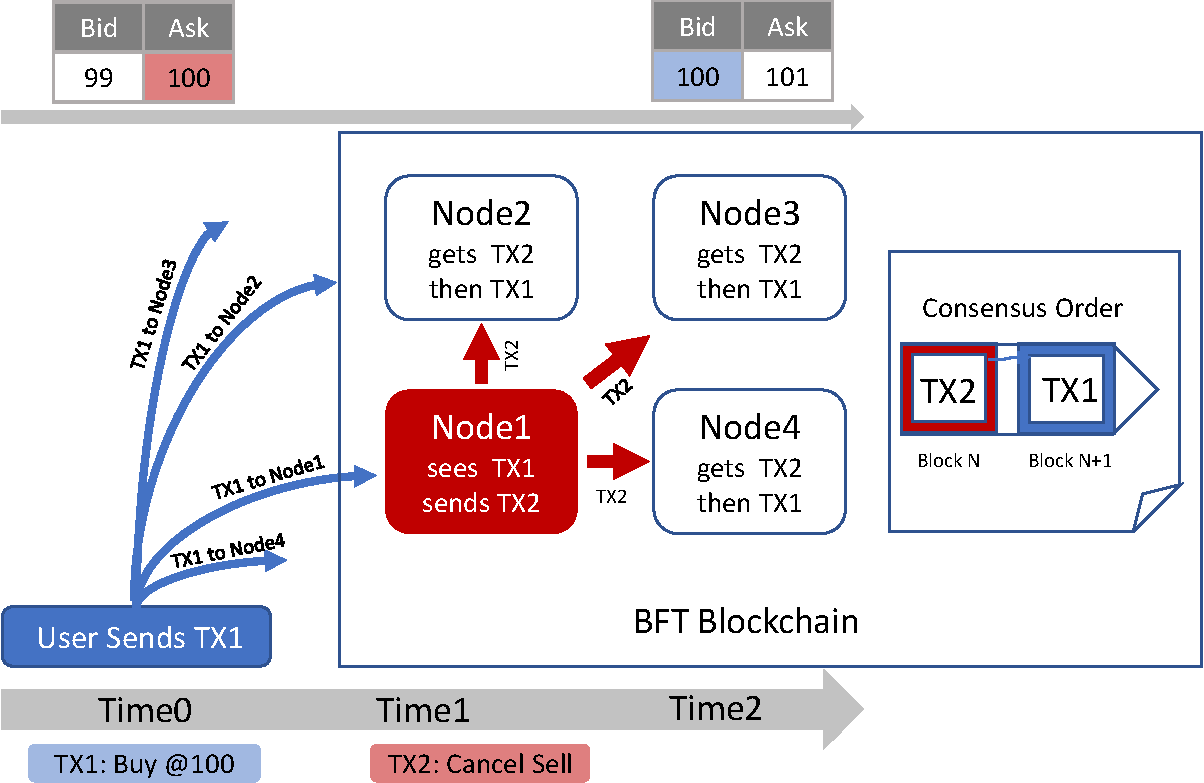
\includegraphics[scale=0.4]{frontrunning3-crop.pdf}
  \caption{Frontrunning in BFT Blockchain - Node1 reads the Users Transaction - \emph{TX1}, and Front runs them with \emph{TX2}, creating \emph{Adverse Selection Risk} for the User}\label{fig:front-running}
\end{figure}

\paragraph{Other work describe similar problems in various ways.} Eskandari et al. \cite{Eskandari} detail the theoretical problems of front-running on \emph{Ethereum} \emph{smart contract limit order book}, and describe \emph{cancellation grief}, for when a cancel transaction is front-run and the  original order gets executed. 

There is empirical evidence of front-running on Ethereum, with Dian concluding that this "poses a realistic threat to Ethereum today". \cite{Daian} 

Luu et al. \cite{Luu} suggest that \emph{Transaction-Ordering Dependence} is an anti-pattern, while others highlight \emph{incentive and ordering attacks} in \emph{POW} blockchains \cite{Judmayer} \cite{Delmolino}. 

Other works discussing front-running in blockchain markets: \cite{Malinova,Eskandari,Clark,Berg}.

\paragraph{Permissioned Blockchains} use well researched \emph{Byzantine Fault Tolerant} (BFT) protocols with \emph{safety} and \emph{liveness} guarantees for distributed state replication. \cite{Gueta} These protocols are meant to be fault tolerant given an assumption of the distribution of honest nodes. However, research has been uncovering new types on non Byzantine attacks or faults:      
\begin{center}
\begin{itemize}{}
  \item \emph{Rational Users} \cite{Hou}
  \item \emph{Alive-but-corrupt} \cite{Malkhi}
  \item \emph{Rational Manipulation} \cite{Shneidman}
  \item \emph{Covert Adversaries} \cite{Aumann}
  \item \emph{Byzantine-Altruistic-Rational (BAR)} \cite{Aiyer}
\end{itemize}
\end{center}

\paragraph{Transaction-order-fairness} as a third Byzantine consensus property guarantee is described in the \emph{Aequitas} protocols \cite{Kelkar_2020}. A graph of all nodes transaction ordering is generated, which does in fact, reach consensus on a weaker form of \emph{order fairness}. However, as described in the paper, the \emph{Condorcet paradox} creates an impossibility for total fair ordering on transactions that have \emph{non transitive} ordering preferences. 

Even in the \emph{Aequitas} protocol, these transactions are left up to protocol developer for ordering. Unfortunately, with front-running on decentralized limit order books, consensus is needed on the orderings of precisely these transactions that are impossible to order! 

\subsubsection*{Why does it not work?} 
\begin{itemize}{}
\item Ethereum abstracted the Bitcoin design into a blockchain, and added a virtual machine and turning complete smart contract language. 
\item Permisssioned blockchains abstracted Bitcoin into Nakamoto consensus and added the rigour of security guarantees from the BFT consensus mechanisms of state replication. 
\item Aequitas solved consensus on abstract transaction ordering consensus protocols. 
\end{itemize}

Only when looking at Bitcoin, and asking ``But why does work?'', as Badertscher et al. \cite{badertscher2018but} does, do we find our answer. They analyze Bitcoin from a Rational Protocol Design (RDP) framework, which is useful for analysing protocols that are already running. It does this by looking at it from the perspective of the protocol design intent and utility vs the utility of a potential adversary.  

\textit{Bitcoin works because it was designed for the specific utility of peer-to-peer electronic cash, and the main goal of its blockhchain design was to create a incentive based equilibrium for preventing double-spends in a censorship resistant way}. \cite{Nakamoto}

\paragraph{Blockchain abstractions as an anti-pattern}
\begin{itemize}{}
\item Ethereum is designed to run any abstract protocol. Yet protocols with order-dependency simply do not work. What went wrong is the abstraction from Bitcoin to blockchain. As the Bitcoin protocol is designed to prevent double spends and double-spend transactions are mutually exclusive. So one should only expect the small set of protocols, to be viable on Ethereum.    

\item BFT consensus protocols were designed for replicating state for a single entity running distributed databases. Abstract multi-party competitive economic incentive based consensus protocols, have no relation to the BFT fault guarantees. 

\end{itemize}

\section*{A New Blockchain Abstraction}
We design our decentralized exchange for its specific utility. First and for-most the utility of exchange is reaching an equilibrium of price discovery. Price is the public good that should come out of our DEX. 

\subsection*{Distributed Mechanism Design}
Pre-dating blockchain, \emph{Algorithmic Game Theory} uses computer science to model complex game  dynamics for \emph{Nash Equilibrium} \cite{nisan_roughgarden_tardos_vazirani_2007}. See Lie et al, for in-depth analysis of Game Theory in Blockchain, with insight into its application to Permissioned blockchains \cite{Liu}.  

\emph{Mechanism design} inverts algorithmic game theory. Where mechanisms are used to design systems and protocols, with actors reaching Nash Equilibrium that are in-line with specific objectives. \cite{nisan_2007} \cite{Shneidman} \cite{DBLP:journals/corr/abs-1905-08595}

Most interesting to us is \emph{Distributed Mechanism Design} applied to Blockchain. Its been used to study centralization issues in blockchains \cite{Ray}, and miner incentives \cite{Chen}.  A recent blog post by Alex Evans, gives a comprehensive overview on \emph{Mechanism Design for Blockchain}, including  \emph{The Revelation Principle} as well as \emph{Vickrey-Clarke-Groves} auctions. \cite{Evans}

\subsection* {Methodology}
Using distributed mechanism design theory, we design our DEX for the purpose of providing the specific utility of price discovery. The design goal is to properly incentivize traders and market-makers to reach an equilibrium which stays within the rules and intent of the protocol, rather than attempt adversarial attacks.

Our utility, price discovery, is itself an equilibrium, and is not easily quantified. Only after building and launching the model in the real world, can we then analyze the data and the running system to measure success. As such, this paper is the first step, to be followed by a real world implementation as a Bitcoin sidechain distributed exchange, Sidepit. 

\subsection* {Tools}
\paragraph{Covert adversaries} describes an adversary that is only incentivized to cheat when they cannot get caught \cite{Aumann}. A deterrent for these attacks come from increased transparency, which is the hallmark feature of protocols dating back to Stornetta and Harbors linked-timestamps, the precursor to blockchain. \cite{10.1007/3-540-38424-3_32} 

\paragraph{Decentralized matching engines} with limit order books is the market mechanism for our exchange. Years of empirical evidence in traditional markets have converged on this process, and we see no reason to re-invent this mechanism. 

\paragraph{Aequitas Transaction Order Fairness} protocol is used, but not for real-time consensus, the transaction ordering consensus graph is generated in the background, for the purpose of spotting adversaries after the fact. This information is a mechanism to disincentivise \emph{covert adversaries} and can be used as reputation based system for quorum slice tier node selection, for our consensus protocol below.    

\section{Fair Price Discovery} 
We define \emph{Fair price discovery} as an exchange with price discovery that is open for anyone to fully participate. We achieve this by removing the time advantage given to \emph{HFT bots} in centralized exchanges. The core solution is a front-running resistant distributed limit order book.  

\subsection*{Decentralized Limit Order Books}
We start with a closed network of exchange nodes, where each node has a matching-engine and maintains a CLOB, like a centralized exchange. 

The distributed network of nodes come to consensus on the total ordering of transactions. This is done in two steps: 

\begin{enumerate}
    \item \emph{block-data} consensus is reached every N seconds on the full list of transactions from the mempool. 
    \item \emph{block-order} consensus is reached via auction on each block, where the highest bidder gets to reorder the transactions in the \emph{block-data} 
\end{enumerate}

From these two simple steps we have removed the advantage of HFT co-location, the need to front-run and overt \emph{Miner Extracted Value} (MEV) through manipulation of ordering or inclusion of transactions.

\paragraph*{HFT Co-location} is no longer possible as there is no single location for the matching engine. Furthermore, the notion of \emph{being first} goes away, as all orders within the block are the same in regards to time. Also, since you can pay to \emph{be first}, after the fact, there is no longer justification of cost of the HFT arms race. 

\paragraph*{Front-running} by \emph{rushing} has no advantage, as the processing order is not determined by which transaction was seen first on the network. 

\paragraph*{Miner Extracted Value} is no longer possible, as we come to consensus on the entire mempool, for each block. Recall, that \emph{MEV} is defined as a miner choosing, ordering or adding new transactions into a block in a way that generates economic value. In our model, each block contains all the outstanding transactions, and the transactions in \emph{block-data} are in no particular order for processing, until after the \emph{block-order} auction. 

\subsection*{Permissioned DEX}
The permissioned DEX is basically just a  centralized exchange with a distributed matching engine. Each member/trader of the exchange gets a full node, and forms a closed p2p network. Consensus on the mempool is reached every ~1 second via a BFT protocol, to create the \emph{block-data}. An auction is run after each block, and the highest bidder pays the exchange the bid amount, and gets to reorder the transactions into the \emph{block-order}. 

As this is all happening in real time, each node will have multiple possible states based of different permutations of the orderings within the \emph{block-data}, but also the new orders coming in. The new orders them-self, create new permutations. 

\paragraph*{This is akin to virtual co-location,} since after the block-data we allow nodes to pay to reorder the transactions into the final \emph{block-order}. This final \emph{block-order}, would be as if they were a co-located \emph{HFT bot} in a centralized exchange with the fasted reaction time. Only now, there is no longer a need for \emph{flashing} orders in fear of \emph{adverse selection}. 

\subsection*{Open DEX}
For a full decentralized implementation, we implement \emph{Sidepit} as a Bitcoin sidechain.  

\begin{enumerate}[leftmargin=*]
\item We move/wrap bitcoin into the sidechain \footnote{either with 1way-peg, drivechain, or a trust minimized federation}, and enable full UTXO coin transfers. 
\item Once in our own sidechain we implement a 2 way peg from our sidechain into the Sidepit exchange, for deposits and withdrawls. 
\item Sidepit uses an account based model, rather than UTXOs 
\item We define an on-chain USD futures contract denominated in Bitcoin, with optional off-chain delivery. \footnote{Delivery cannot be enforced, but can  be connected to OTC DEXs like \emph{bisq}}  
\item We define \emph{exchangeOrder} transactions that can be a buy/sell/cancel with limit or market price.
\item Every ~1 second the \emph{Sidepit federated consensus protocol} comes to consensus on the \emph{block-data} containing \emph{exchangeOrders}
\item The \emph{block-order} auction is done by signing a modified version of covenant transactions \footnote{See https://gist.github.com/RubenSomsen/5e4be6d18e5fa526b17d8b34906b16a5}, making a chain of payments each second until the next bitcoin block.     
\item A list of \emph{block-data} is processed in \emph{block-order} by each node, resulting in the state of full exchange order book, complete will positions, fills and PnL. Each node updates all the accounts balances, as this is deterministic.  
\item Each Bitcoin block will contain a special Sidepit transaction, which includes a merkle root of a chain of \emph{block-data}:\emph{block-order} pairs, representing each ~1 second block of \emph{exchangeOrder} transactions, as well as the payment from the \emph{block-order} auctions for each block. \footnote{Bitcoin miners are paid, as they represent a Sybil resistant set unlikely to have an interest in front-running the \emph{block-data}. Note: unlike MEV, all they can accomplish is a free reordering, by paying them-self. Alternatively, the payment can be burnt, paid to a federation} 
\item A valid Sidepit hash finalizes the state of the DEX, while an invalid one, only creates a hard-fork and a pause, only resulting in loss of bitcoin for attacker. \footnote{Since honest nodes will only bid to reorder a valid hash, an attacker would have to pay more than all auctions since the last Bitcoin block combined.}
\end{enumerate}

\subsubsection*{Sidepit Federated Consensus Protocol (SFCP) } 
SFCP is a modified Stellar Consensus Protocol \cite{thestellar} which is a Federated Byzantine Agreement protocol. \\

Borrowing the ideas described by David Mazières \cite{thestellar}, we note that a DEX is like the internet in that ``Transitively, everyone wants to talk to everyone''. While trader nodes maybe in a competition, and even adversarial to each other, they require \emph{all} transactions from all peers to pass into their local mempool matching engine, and create a CLOB state, in order to make trading decisions and sign/gossip new transaction orders.        

\paragraph{A Tiered Quorum Slice} model is used, where each node chooses set of nodes for real-time BFT consensus every ~1 second, similar to the permissioned model. The protocol reaches consensus as long as there is quorum slice overlap. This must come from social consensus and requires a \emph{Weak Subjectivity}.   

\paragraph{Hypothesis: DEX trader relationships transitively converge.} Market makers, high volume traders, and exchanges are the tier1 ISP equivalent of DEX. Eventually market forces should converge on honest, high volume, stable up-time, and well known nodes to use as tier1 for quorum slices.

\subsubsection*{On-Chain Settlement}
Any DEX with on-chain matching needs a token for margin and settlement, otherwise fills from matching in the order-book can not be guaranteed. Guaranteed settlement of fills, is a basic requirement for price-discovery in open markets. Atomic swaps, for example, cannot guarantee settlement, they can only guarantee no funds are lost, in case one party reneges. Sidepit uses pegged bitcoin for on-chain margin and settlement of a USD futures contract priced in bitcoin.    
 
\newpage
\bibliography{sidepit}{}
% \bibliographystyle{plain}
\bibliographystyle{unsrt}

\end{document}